\documentclass{beamer}
\usepackage{minted}
\usepackage{graphicx}
\usepackage{hyperref}
\usetheme{Madrid}

\definecolor{RedOrange}{rgb}{1,0.3,0}

\author{Clarissa Littler}
\title{Making Websites for Beginners}
\date{}

\begin{document}
\setbeamercovered{transparent}

\begin{frame}
\maketitle
\end{frame}

\section{What is this class?}
\begin{frame}{What we'll cover}
  \begin{itemize}
    \item The basic technology that goes into a webpage \pause
    \item Simple examples of how to use HTML and CSS \pause and \alert{maybe} a little JavaScript \pause
    \item Resources to continue your learning
  \end{itemize}
\end{frame}

\begin{frame}{What we won't cover}
  \begin{itemize}
    \item How to build the back-end of a site \pause
    \item How to program in JavaScript in general \pause
      \begin{itemize}
        \item Though there are free supplements for that \pause
      \end{itemize}
    \item A majority of CSS and HTML
  \end{itemize}
\end{frame}
\section{What is a website?}
% at some point I should replace this with pictures because it's too wordy
\begin{frame}{Client and server}
  \begin{block}{}
    Two pieces that talk to each other to make a site
  \end{block}
  \begin{columns}
    \begin{column}{0.4\columnwidth}
      \begin{block}{Server}
        \begin{itemize}
          \item<1-> \textcolor<2>{RedOrange}{Sends data to the browser}
          \item<1,3-> \textcolor<3>{RedOrange}{Saves information for long term use}
          \item<1,4-> \textcolor<4>{RedOrange}{Receives requests from the client}
        \end{itemize}
      \end{block}
    \end{column}

    \begin{column}{0.4\columnwidth}
      \begin{block}{Client}
        \begin{itemize}
          \item<1,5-> \textcolor<5>{RedOrange}{Receives data from the server}
          \item<1,6-> \textcolor<6>{RedOrange}{Renders server data into a usable page}
          \item<1,7-> \textcolor<7>{RedOrange}{Handles the user interface}
        \end{itemize}
      \end{block}
    \end{column}
  \end{columns}
\end{frame}

\begin{frame}{How do you share a site?}
  \begin{block}{}
    \begin{itemize}
      \item<1-> You can load a site locally in your browser
      \item<2-> To share a site you need a server to \alert{host}
      \item<3-> Free hosting option: \url{neocities.org}
    \end{itemize}
  \end{block}
\end{frame}

\begin{frame}{The three pieces of a web page}
\begin{itemize}
  \item HTML \pause
  \item CSS \pause
  \item JavaScript
\end{itemize}
\end{frame}

\begin{frame}{HTML}
  \begin{block}{What does HTML do?}
    HTML describes the content of the page, \pause \textcolor{RedOrange}{but not how it looks}
  \end{block}
\end{frame}

\begin{frame}{CSS}
  \begin{block}{What does CSS do?}
    CSS describes how a page looks, \pause \textcolor{RedOrange}{but not its content}
  \end{block}
\end{frame}

\begin{frame}{JavaScript}
  \begin{block}{What does JavaScript do?}
    The dynamics and the user interface of the page
  \end{block}
\end{frame}
\section{Basic HTML}

\begin{frame}{What \alert{is} HTML?}
  \begin{block}{HyperText Markup Language}
      \begin{itemize}
        \item HyperText \pause
        \item Markup
      \end{itemize}
  \end{block}
\end{frame}

\begin{frame}[fragile]{Tags and Elements}
  \begin{block}{}
    \begin{semiverbatim}
\onslide<1-2> <body>
\onslide<1,3>  <h1>This is a heading</h1>
\onslide<1,4>  <p>
\onslide<1,5>      This is a paragraph of text, 
\onslide<1,5,6>      where some of the text is <b>bold</b>, and
\onslide<1,5>      after this paragraph, there will be a numbered list
\onslide<1,4>  </p>

\onslide<1,7>  <ol>
\onslide<1,8>    <li>lists are made of "list items"</li>
\onslide<1,8>    <li>like these</li>
\onslide<1,7>  </ol>
\onslide<1-2> </body>
    \end{semiverbatim}
  \end{block}
\end{frame}

\setbeamercovered{invisible}
\begin{frame}[fragile]{Whence closing tags}
  \begin{block}{}
    \begin{semiverbatim}
      <body>
        <ol>
          <li>This is a list\onslide<2,3>{</li>}
          <li>but\onslide<2,3>{</li>}
          <li>there's ambiguity here\onslide<2>{</li>}
        \onslide<2>{</ol>}
        <ol>
         <li> where does this part go?\onslide<2,3>{</li>}
         <li> is it a sublist or a second list?\onslide<2,3>{</li>}
        \onslide<2,3>{</ol>}
        \onslide<3>{</li>}
        \onslide<3>{</ol>}
    \end{semiverbatim}
  \end{block}
\end{frame}
\setbeamercovered{transparent}

\begin{frame}[fragile]{Whence closing tags}
  \begin{columns}
    \begin{column}{0.4\columnwidth}
      \begin{block}{}
        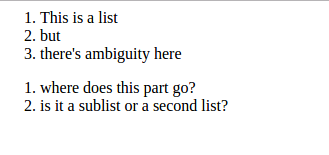
\includegraphics[width=.9\linewidth]{noClose1}
      \end{block}
    \end{column}
    \begin{column}{0.4\columnwidth}
      \begin{block}{}
        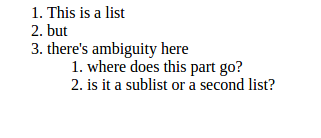
\includegraphics[width=.9\linewidth]{noClose2}
      \end{block}
    \end{column}
  \end{columns}
\end{frame}

\begin{frame}[fragile]{The basic template}
 \begin{block}{}
  \begin{semiverbatim}
   \onslide<1,2><!doctype html>
   \onslide<1,3><html>
   \onslide<1,4>  <head>
       ...
   \onslide<1,4>  </head>
   \onslide<1,5>  <body>
       ...
   \onslide<1,5>  </body>
   \onslide<1,3></html>
  \end{semiverbatim}
 \end{block}
\end{frame}

\begin{frame}[fragile]{Headings}
  \begin{columns}
    \begin{column}{0.45\columnwidth}
      \begin{block}{}
        \begin{minted}[]{html}
<!doctype html>
<html>
  <body>
    <h1>Big heading</h1>
    <h2>Smaller</h2>
    <h3>Smaller</h3>
    <h4>Even smaller</h4>
    <h5>Smallller</h5>
    <h6>Smallest</h6>
  </body>
</html>
        \end{minted}
      \end{block}
    \end{column}
    \begin{column}{0.45\columnwidth}
      \begin{block}{}
        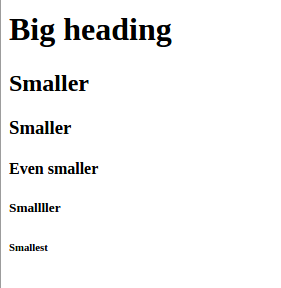
\includegraphics[width=.9\linewidth]{headings.png}
      \end{block}
    \end{column}
  \end{columns}
\end{frame}

\begin{frame}[fragile]{Lists}
  \begin{block}{}
    \begin{minted}[]{html}
<!doctype html>
<html>
  <body>
    <ol>
      <li>This is an ordered list</li>
      <li>And here we have a nested list
	<ul>
	  <li>and this is an unordered list</li>
	  <li>which is by default</li>
	  <li>a bulleted list</li>
	</ul>
      </li>
    </ol>
  </body>
</html>
    \end{minted}
  \end{block}
\end{frame}

\begin{frame}{Lists}
  \begin{block}{}
    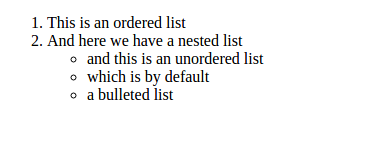
\includegraphics[width=9cm]{listylists.png}
  \end{block}
\end{frame}

\begin{frame}[fragile]{Exercise 1}
\begin{columns}
\begin{column}{0.4\columnwidth}
  \begin{block}{}
    Let's try making a simple web page ourselves!
    \begin{itemize}
      \item Open notepad++
      \item Type along the instructions
      \item Save the file in the F drive (end the file in .html)
      \item Right click and open in the browser
    \end{itemize}
  \end{block}
\end{column}
\begin{column}{0.5\columnwidth}
\setbeamercovered{invisible}
  \begin{semiverbatim}
\onslide<2-> <!doctype html>
\onslide<3-> <html>
\onslide<4->  <body>
\onslide<5->   <h1>This is our heading</h1>
\onslide<6->   <p>Here is our text.</p>
\onslide<7->   <p>Here's more <b>text</b></p>
\onslide<8->  </body>
\onslide<9-> </html>
  \end{semiverbatim}
\setbeamercovered{transparent}
\end{column}
\end{columns}
\end{frame}

\begin{frame}[fragile]
  \begin{block}{Exercise 2}
    Try making your own simple page using
    \begin{itemize}
      \item \Verb"<p>"
      \item \Verb"<h1>"
      \item \Verb"<ol>"
      \item \Verb"<ul>"
      \item \Verb"<li>"
    \end{itemize}
    tags, following the process of the last example
  \end{block}
\end{frame}

\begin{frame}[fragile]{Anchors and Attributes}
 \begin{block}{}
   \texttt{<a href="https://multcolib.org">This is a link</a>}
 \end{block}
\end{frame}

\begin{frame}{Exercise 3}
  \begin{block}{}
    {\Large
      Create your own page that uses at least two links and test them to ensure they work
    }
  \end{block}
\end{frame}

\section{CSS}

\begin{frame}{Cascading Style Sheets}
  \begin{block}{What is CSS?}
    Cascading style sheets control the appearance of elements
  \end{block}
\end{frame}

\begin{frame}[fragile]{CSS Entries}
  \begin{block}{}
    \begin{semiverbatim}
\onslide<1,2>selector \{
\onslide<1,3>    property: value;
\onslide<1,3>    property: value;
\onslide<1,3>    property: value;
\onslide<1,2>\}
     \end{semiverbatim}
   \end{block}
\end{frame}

\begin{frame}[fragile]{Adding CSS to a page}
 \begin{block}{Style tags}
\begin{semiverbatim}
\onslide<1><!doctyle html>
\onslide<1><html>
\onslide<1>  <head>
\onslide<1,2>    <style>
\onslide<1>      ...
\onslide<1,2>    </style>
\onslide<1>  </head>
\onslide<1>  <body>
\onslide<1>    ...
\onslide<1>  </body>
\onslide<1></html>
\end{semiverbatim}
\end{block}
\end{frame}

\begin{frame}[fragile]{Selecting elements by ID}
 \begin{block}{}
\begin{semiverbatim}
\onslide<1><!doctype html>

\onslide<1><html>
\onslide<1>  <head>
\onslide<1,2>    <style>
\onslide<1-3>      #para \{
\onslide<1-4>         color: blue;
\onslide<1-3>      \}
\onslide<1,2>    </style>
\onslide<1>  </head>
\onslide<1>  <body>
\onslide<1>    <p id="para">This is the text within our paragraph.</p>
\onslide<1>  </body>
\onslide<1></html>
\end{semiverbatim}
\end{block}
\end{frame}

\begin{frame}{Selecting elements by ID}
  \begin{block}{}
    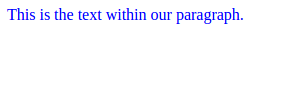
\includegraphics[width=5cm]{byId.png}
  \end{block}
\end{frame}

\begin{frame}[fragile]{Exercise 4}
\begin{columns}
  \begin{column}{0.3\columnwidth}
    \begin{block}{Let's use CSS}
      \begin{itemize}
      \item Open a new file in the text editor
      \item Copy the template on this slide
      \item Fill in the style element within the \Verb"<head>" tags
      \item Turn the middle heading green
      \end{itemize}
    \end{block}
  \end{column}

  \begin{column}{0.6\columnwidth}
    \begin{block}{}
      \begin{semiverbatim}
<!doctype html>
<html>
  <head>
    <style>
      fill this in
    </style>
  </head>
  <body>
    <h1 id="heading1">First</h1>
    <h2 id="heading2">Second</h2>
    <h3 id="heading3">Third</h3>
  </body>
</html>
      \end{semiverbatim}
    \end{block}
  \end{column}
\end{columns}
\end{frame}

\begin{frame}{Selecting elements by ID}
\begin{block}{}
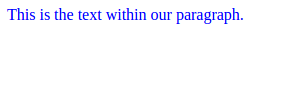
\includegraphics[width=5cm]{byId.png}
\end{block}
\end{frame}

\begin{frame}[fragile]{Selecting elements by class}
 \begin{block}{}
\begin{minted}[]{css}
.ourClass {
    color: red;
    width: 200px;
    font-weight: bold;
}
\end{minted}
\end{block}
\end{frame}

\begin{frame}[fragile]{Selecting elements by class}
 \begin{block}{}
\begin{minted}[]{html}
<p class="ourClass">Here's the 
text in one paragraph. 
There's going to be a fair 
decent length of text here so we 
can see that the width 
restriction causes the text to wrap around.</p>

<ol class="ourClass">
  <li>Here's a list here that's 
  also going to have an item 
  with at least a moderately long 
  single element 
  in order to show the 
  effects of the width property</li>
</ol>
\end{minted}
\end{block}
\end{frame}

\begin{frame}{Selecting elements by class}
\begin{block}{}
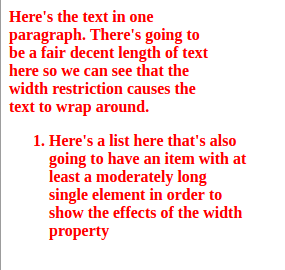
\includegraphics[width=5cm]{byClass.png}
\end{block}
\end{frame}

\begin{frame}[fragile,label={sec:orgheadline34}]{Exercise 5}
 \begin{block}{}
{\Large
Open a new file, follow the template on this slide, then add in CSS declarations to make both paragraphs have \texttt{width: 200px} and the first paragraph have a color of \texttt{blue}
}
\end{block}
\begin{block}{}
\begin{minted}[]{html}
<!doctype html>
<html>
  <head>
  </head>
  <body>
    <p class="theClass" id="firstPara">
    This is a paragraph that has some text in it 
    and, y'know, stuff and things</p>
    <p class="theClass" id="sndPara">
      This is the second paragraph by gum</p>
  </body>
</html>
\end{minted}
\end{block}
\end{frame}

\begin{frame}[fragile]{Selecting elements by type}
 \begin{block}{}
\begin{minted}[]{css}
p {
    font-size: large;
    background-color: green;
    color: blue;
    width: 200px;
}
\end{minted}
\end{block}
\end{frame}

\begin{frame}[fragile,label={sec:orgheadline36}]{Selecting elements by type}
 \begin{block}{}
\begin{minted}[]{html}
<p>Our first paragraph is here. 
  There's some text and things of that ilk.</p>
<p>This is our second paragraph, 
  beholden to no one but itself. 
  A wild rebel of a paragraph</p>
<p>Our third paragraph lies here, 
  relentless in its comformity. 
  There's not much to say about ol' thirdy, 
  they're simply stoic and 
  resolute in their paragraphness.</p>
\end{minted}
\end{block}
\end{frame}


\begin{frame}{Selecting elements by type}
\begin{block}{}
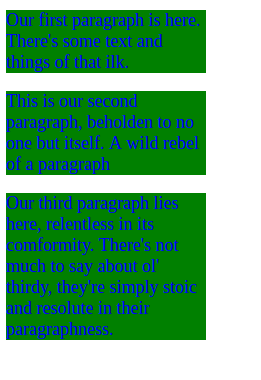
\includegraphics[width=5cm]{byType.png}
\end{block}
\end{frame}

\begin{frame}[fragile]{Specificity}
 \begin{block}{combining type and class}
\begin{minted}[]{css}
p {
    font-size: large;
    background-color: green;
    color: blue;
    width: 200px;
}
p.rebel {
    width: 300px;
    background-color: white;
}
\end{minted}
\end{block}
\end{frame}

\begin{frame}[fragile]{Specificity}
 \begin{block}{}
\begin{minted}[]{html}
<h1 class="rebel">This time we also have a rebellious heading, 
which should be unchanged</h1>

<p>Our first paragraph is here.
  There's some text and things of that ilk.</p>
<p class="rebel">This is our second paragraph, 
  beholden to no one but itself. 
  A wild rebel of a paragraph</p>
<p>Our third paragraph lies here,
  relentless in its comformity. 
  There's not much to say about ol' thirdy, 
  they're simply stoic and resolute
  in their paragraphness.</p>
</div>
\end{minted}
\end{block}
\end{frame}

\begin{frame}{Specificity}
\begin{block}{}
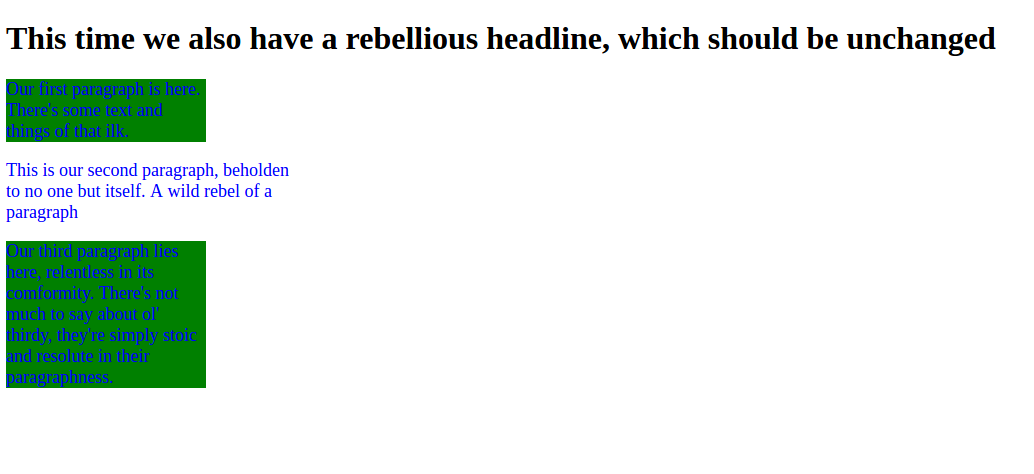
\includegraphics[width=11cm]{specific.png}
\end{block}
\end{frame}

\begin{frame}{Div and span}
  \begin{block}{}
    \begin{itemize}
      \item Div and span are used to group related elements together
      \item {\itshape But they don't have an appearance themselves}
    \end{itemize}
  \end{block}
\end{frame}

\begin{frame}[fragile]{Specificity}
 \begin{block}{choosing children of an element}
\begin{minted}[]{css}
#divvy p{
  width: 200px;
  font-weight: bold;
}
\end{minted}
\end{block}
\end{frame}

\begin{frame}[fragile]{Specificity}
 \begin{block}{choosing children of an element}
\begin{minted}[]{html}
<div id="divvy">
  <p> Here we're going to have some text </p>
  <p> and a little more even, in a separate paragraph. </p>

  <ul>
    <li>but this shouldn't be effected by our code at all</li>
  </ul>
</div>
<p>Neither should anything in here, either</p>
\end{minted}
\end{block}
\end{frame}
\begin{frame}[label={sec:orgheadline46}]{Specificity}
\begin{block}{}
\includegraphics[width=.9\linewidth]{childExample.png}
\end{block}
\end{frame}
\begin{frame}[fragile,label={sec:orgheadline47}]{Exercise 6}
 \begin{block}{}
{\large
Using the following skeleton, found in \texttt{exer6.html}, add CSS declarations so that the first paragraph has \emph{blue} text, the second paragraph has \emph{red} text, and the third paragraph has \emph{green} text.
}
\end{block}
\begin{block}{}
\begin{minted}[]{html}
<body>
  <p>our first paragraph</p>
  <div>
    <p>our second paragraph</p>
    <div>
      <p>our third paragraph </p>
    </div>
</body>
\end{minted}
\end{block}
\end{frame}


\section{JavaScript}

\begin{frame}{What is the Document Object Model?}
  \begin{block}{}
    The Document Object Model (DOM) gives you the ability to write \alert<2>{code} that changes the \alert<3>{web page} \alert<4>{dynamically} 
  \end{block}
\end{frame}

\begin{frame}{What does the DOM do?}
  \begin{block}{}
    \begin{itemize}
    \item Change CSS classes \pause
    \item Create and remove HTML elements \pause
    \item Respond to user interface \alert<4>{events}
    \end{itemize}
  \end{block}
\end{frame}

\begin{frame}{What is JavaScript?}
  \begin{block}{}
      JavaScript is a programming language \pause that runs in the browser
  \end{block}
\end{frame}

\begin{frame}{What are programming languages?}
  \begin{block}{A programming language is\ldots{}}
    \begin{itemize}
    \item a formal language with rules and grammar \pause
    \item that has meaning as computation \pause
    \item and can be used to talk to a computer
    \end{itemize}
  \end{block}
\end{frame}

\begin{frame}[fragile]{Script tag}
 \begin{block}{}
\begin{semiverbatim}
\onslide<1><!doctype html>

\onslide<1><html>
\onslide<1>  <head>
\onslide<1,2>    <script>
\onslide<1,2,3>      ...
\onslide<1,2>    </script>
\onslide<1>  </head>
\onslide<1>  <body>
\onslide<1>    ...
\onslide<1>  </body>
\onslide<1></html>
\end{semiverbatim}
\end{block}
\end{frame}

\begin{frame}{JavaScript console}

\includegraphics[width=.9\linewidth]{console.png}
\end{frame}

\begin{frame}{Basic programming constructs}
  \begin{columns}[T]
    \begin{column}{0.4\columnwidth}
      \begin{block}{Data}
        \begin{itemize}
          \item<1,2,3> Numbers
          \item<1,2,4> Text
          \item<1,2,5> Lists
          \item<1,2,6> Dictionaries
        \end{itemize}
      \end{block}
    \end{column}
    \begin{column}{0.4\columnwidth}
      \begin{block}{Actions}
        \begin{itemize}
          \item<1,7,8> Arithmetic
          \item<1,7,9> Creating and using storage
          \item<1,7,10> Performing actions multiple times
          \item<1,7,11> Making choices about what to do
          \item<1,7,12> Naming routine tasks to easily perform them again
        \end{itemize}
      \end{block}
    \end{column}
  \end{columns}
\end{frame}

% \begin{frame}[fragile]{Arithmetic}
%   \begin{columns}
%     \begin{column}{0.4\columnwidth}
%       \begin{block}{Numbers}
%         \begin{itemize}
%         \item 1
%         \item 0.5
%         \item -20
%         \item \(\ldots\)
%         \end{itemize}
%       \end{block}
%     \end{column}
%     \begin{column}{0.4\columnwidth}
%       \begin{block}{Operations}
%         \begin{itemize}
%         \item \texttt{+}
%         \item \texttt{-}
%         \item \texttt{*}
%         \item \(\ldots\)
%         \end{itemize}
%       \end{block}
%     \end{column}
%   \end{columns}
% \end{frame}

% \begin{frame}{Arithmetic Exercise}
% \begin{block}{Exercise}
%   Open your console and type the following expressions:
%   \begin{itemize}
%     \item $10 + 20$
%     \item $100 / 2$
%     \item $100 - 100 - 100$
%   \end{itemize}
% \end{block}
% \end{frame}

\begin{frame}[fragile]{Strings}
 \begin{columns}[T]
   \begin{column}{0.4\columnwidth}
     \begin{block}{}
       Strings are text-as-data, useful for:
       \begin{itemize}
         \item<1,2> error messages
         \item<1,3> writing output
       \end{itemize}
     \end{block}
   \end{column}
   \begin{column}{0.5\columnwidth}
     \begin{block}{}
       \begin{semiverbatim}
 \onslide<1,4>"this is a string"
 \onslide<1,5>'this is also a string'
 \onslide<1,6>"even this 'is a string'"
       \end{semiverbatim}
     \end{block}
   \end{column}
 \end{columns}
\end{frame}

\begin{frame}[fragile]{Strings exercise}
  \begin{block}{}
    Type the following into the console:
    \begin{itemize}
      \item \texttt{"hi there everybody"}
      \item \texttt{"it's such a 'nice' day"}
      \item \texttt{"I'm in this class" + " and I'm typing"}
    \end{itemize}
  \end{block}
\end{frame}


\begin{frame}[fragile]{Variables and Storage}
  \begin{columns}[T]
    \begin{column}{0.4\columnwidth}
      \begin{block}{Variables...}
        \begin{itemize}
          \item<1,2> are names given to data
          \item<1,3> are storage containers
          \item<1,4> can change in value
        \end{itemize}
      \end{block}
    \end{column}

    \begin{column}{0.5\columnwidth}
      \begin{block}{Type along}
\begin{semiverbatim}
\onslide<1,5>var thisVariable="a string"
\onslide<1,6>thisVariable
\onslide<1,7>thisVariable = 10
\onslide<1,8>thisVariable
\end{semiverbatim}
      \end{block}
    \end{column}
  \end{columns}
\end{frame}

\begin{frame}[fragile]{Lists and Arrays}
\begin{block}{}
    In JavaScript, the data type for lists are called \alert{arrays}
\end{block}
\begin{columns}[T]
  \begin{column}{0.4\columnwidth}
    \begin{block}{Arrays}
    \begin{itemize}
      \item<1,2> have a beginning and end
      \item<1,3> are in order
      \item<1,4> can be accessed by index
    \end{itemize}
    \end{block}
  \end{column}
  \begin{column}{0.4\columnwidth}
    \begin{block}{Type along}
      \begin{semiverbatim}
\onslide<1,5>var myArr = [1,2,3]
\onslide<1,6>myArr
\onslide<1,7>myArr[0]
\onslide<1,8>myArr[1]
\onslide<1,9>myArr[2]
\onslide<1,10>myArr[0] = 20
\onslide<1,11>myArr[0]
      \end{semiverbatim}
    \end{block}
  \end{column}
\end{columns}
\end{frame}

% \begin{frame}[fragile]{Arrays exercise}
%   \begin{block}{Type the following}
%     \begin{semiverbatim}
% var myArray = ["fish",10,[1,2,3]]
% myArray[2][0]

%     \end{semiverbatim}
%   \end{block}
% \end{frame}

\begin{frame}[fragile]{Objects and Dictionaries}
  \begin{columns}[T]
    \begin{column}{0.4\columnwidth}
      \begin{block}{Objects...}
        \begin{itemize}
          \item<1,2> are like dictionaries
          \item<1,3> associate names and data
          \item<1,4> are used to collect information
        \end{itemize}
      \end{block}
    \end{column}

    \begin{column}{0.5\columnwidth}
      \begin{block}{Type along}
\begin{semiverbatim}
\onslide<1,5>var obj = \{names : "chicken", 
\onslide<1,5>           petSpecies : "dog", 
\onslide<1,5>           age : 10\}
\onslide<1,6>obj.names
\onslide<1,7>obj.petSpecies
\onslide<1,8>obj.age = 10
\onslide<1,9>obj.age
\end{semiverbatim}
      \end{block}
    \end{column}
  \end{columns}
\end{frame}

\begin{frame}[fragile]{Functions}
  \begin{columns}[T]
    \begin{column}{0.35\columnwidth}
      \begin{block}{Functions...}
        \begin{itemize}
          \item<1,2> are code that can be used again and again
          \item<1,3> are data that can be assigned to variables
          \item<1,4> use the keyword \texttt{return} to give back a value
          \item<1,5> are made up of \alert{arguments} and a \alert{body}
        \end{itemize}
      \end{block}
    \end{column}
    \begin{column}{0.6\columnwidth}
      \begin{block}{}
      \begin{semiverbatim}
\onslide<1,6,7>function () \{ 
\onslide<1,6,7>//this function doesn't have a name
\onslide<1,6,8>   var x = 10;
\onslide<1,6,9>   return x + x;
\onslide<1,6,7>\}

\onslide<1,10,11>function thisFun (x,y) \{ 
\onslide<1,10,11>//but this function does
\onslide<1,10,12>   return (x + y);
\onslide<1,10,11>\}
      \end{semiverbatim}
      \end{block}
    \end{column}
  \end{columns}
\end{frame}

\begin{frame}{How we'll proceed}
  \begin{block}{}
    From here on, we'll be presenting examples of JavaScript interacting with the DOM \pause and practice more JavaScript from there
  \end{block}
\end{frame}

\section{The Document Object Model}

\begin{frame}{What is the Document Object Model?}
  \begin{block}{The DOM}
    The document object model (DOM) is the representation of the web page \emph{as JavaScript objects}
  \end{block}
\end{frame}

\begin{frame}[fragile]{Putting the document in DOM}
 \begin{block}{The document object}
   \texttt{document} is the object that holds most of the important methods for controlling web pages 
 \end{block}
\end{frame}

\begin{frame}{Our first example}
\begin{block}{}
  In our first example we'll
  \begin{itemize}
    \item<1,2> create an HTML element in JavaScript
    \item<1,3> create text to put inside the element
    \item<1,4> insert the HTML element in the web page
  \end{itemize}
\end{block}
\end{frame}

\begin{frame}[fragile]{When to load code}
\begin{block}{}
 \begin{minted}{js}
window.onload = function () {
    ... 
};
\end{minted}
\end{block}
\end{frame}

\begin{frame}[fragile]{Creating elements}

    \begin{block}{Relevant functions}
      \begin{itemize}
        \item \texttt{document.createElement}
        \item \texttt{document.createTextNode}
        \item \texttt{element.appendChild}
        \item \texttt{document.body}
      \end{itemize}
    \end{block}

\end{frame}

\begin{frame}[fragile]{Creating elements}
    \begin{block}{}
      \begin{semiverbatim}
\onslide<1><!doctype html>

\onslide<1><html>
\onslide<1>  <head>
\onslide<1,2>    <script>
\onslide<1,3>      window.onload = function () \{
\onslide<1,4>        var elm = document.createElement("p");
\onslide<1,5>        var text = document.createTextNode("this is text");
\onslide<1,6>        elm.appendChild(text);
\onslide<1,7>        document.body.appendChild(elm);
\onslide<1,3>      \}
\onslide<1,2>    </script>
\onslide<1>  </head>
\onslide<1>  <body>
\onslide<1>  </body>
\onslide<1></html>
      \end{semiverbatim}
    \end{block}
\end{frame}

\begin{frame}[fragile]{Your turn}
\begin{columns}[T]

\begin{column}{0.3\columnwidth}
  \begin{block}{}
    \begin{itemize}
      \item Create a new html file
      \item Leave the body empty
      \item Create two elements and put them in the body
    \end{itemize}
  \end{block}
\end{column}

\begin{column}{0.65\columnwidth}
\begin{block}{}
  \begin{semiverbatim}
\onslide<1><!doctype html>
\onslide<1><html>
\onslide<1>  <head>
\onslide<1>    <script>
\onslide<1,2>      window.onload = function () \{
\onslide<1,2>        ...
\onslide<1,2>      \}
\onslide<1>    </script>
\onslide<1>  </head>
\onslide<1>  <body>
\onslide<1>  </body>
\onslide<1></html>
  \end{semiverbatim}
\end{block}
\end{column}
\end{columns}
\end{frame}


\begin{frame}[fragile]{Getting existing elements}
  \begin{block}{}
    \begin{itemize}
    \item \texttt{document.getElementById} \pause
    \item \texttt{document.getElementsByTagName} \pause
    \item \texttt{element.firstChild} \pause
    \item \texttt{node.nodeValue}
    \end{itemize}
  \end{block}
\end{frame}

\begin{frame}[fragile]{getElementById}
\begin{block}{}
 \begin{minted}[]{html}
<body>
  <ol id="list1">
    <li>This is a list</li>
  </ol>
  <ol id="list2">
    <li>This is our second list</li>
  </ol>
</body>
\end{minted}
\end{block}
\end{frame}

\begin{frame}[fragile]{getElementById}
\begin{block}{}
 \begin{minted}[]{js}
window.onload = function () {
    var newItem = 
      document.createElement("li");
    var newText =
	document
	.createTextNode("item in the second list");
    newItem.appendChild(newText);
    var secondList = document.getElementById("list2");
    secondList.appendChild(newItem);
};
\end{minted}
\end{block}
\end{frame}

\begin{frame}[fragile]{Your turn}
\begin{columns}[T]

\begin{column}{0.3\columnwidth}
  \begin{block}{}
    \begin{itemize}
      \item Create a new html file
      \item Follow the template to the right
      \item Add an element to the list
    \end{itemize}
  \end{block}
\end{column}

\begin{column}{0.65\columnwidth}
\begin{block}{}
  \begin{semiverbatim}
<!doctype html>
<html>
  <head>
    <script>
      window.onload = function () \{
        ...
      \}
    </script>
  </head>
  <body>
    <ol id="list">
    </ol>
  </body>
</html>
  \end{semiverbatim}
\end{block}
\end{column}
\end{columns}
\end{frame}

% \begin{frame}[fragile]{getElementsByTagName}
%  \begin{block}{}
% \begin{minted}[]{html}
% <!doctype html>
% <html>
%   <head>
%     <script src="getElementsByTagName.js"></script>
%   </head>
%   <body>
%     <ol id="list1">
%       <li>This is a list</li>
%     </ol>
%     <ol id="list2">
%       <li>This is our second list</li>
%     </ol>
%   </body>
% </html>
% \end{minted}
% \end{block}
% \end{frame}
% \begin{frame}[fragile,label={sec:orgheadline53}]{getElementsByTagName}
%  \begin{block}{}
% \begin{minted}[]{js}
% window.onload = function () {
%     var lists = document.getElementsByTagName("ol");

%     for(var i = 0; i < lists.length; i = i + 1){
% 	var list = lists[i];
% 	var newItem = document.createElement("li");
% 	var newText = document.createTextNode("new element");
% 	newItem.appendChild(newText);
% 	list.appendChild(newItem);
%     }
% };
% \end{minted}
% \end{block}
% \end{frame}

\begin{frame}[fragile]{Changing CSS properties}
  \begin{block}{Important properties and methods}
    \begin{itemize}
      \item<1,2> \texttt{elm.style}
      \item<1,3> \texttt{elm.classList}
      \item<1,4> \texttt{elm.classList.add}
      \item<1,5> \texttt{elm.classList.remove}
    \end{itemize}
  \end{block}
\end{frame}

\begin{frame}[fragile]{Changing CSS properties}
 \begin{block}{}
\begin{minted}[]{html}
<!doctype html>
<html>
  <head>
    <script>
      window.onload = function () {
	var h = document.getElementById("heading");
	h.style.color = "red";
      }
    </script>
  </head>
  <body>
    <h1 id="heading">This is a heading!</h1>
  </body>
</html>
\end{minted}
\end{block}
\end{frame}

\begin{frame}[fragile,label={sec:orgheadline55}]{Changing the CSS class}
 \begin{block}{}
\begin{minted}[]{html}
<head>
  <style>
    .reddish {
      color: red;
    }
  </style>
  <script>
    window.onload = function () {
       var h = document.getElementById("heading");
       h.classList.add("reddish");
    };
  </script>
</head>
\end{minted}
\end{block}
\end{frame}

\begin{frame}{Events}
\begin{block}{What are events?}
Events connect user interfaces to code
\begin{itemize}
  \item<1,2>Mouse clicks
  \item<1,3>Keys pressed
  \item<1,4>Moving your cursor
  \item<1,5>Focusing on an element
\end{itemize}
\end{block}
\end{frame}

\begin{frame}[fragile]{Events}
  \begin{block}{Listening for events}
    \begin{itemize}
      \item<1,2> \texttt{elem.addEventListener}
      \item<1,3> \texttt{elem.removeEventListener}
    \end{itemize}
  \end{block}
\end{frame}

\begin{frame}[fragile,label={sec:orgheadline57}]{Listening to events}
 \begin{block}{}
\begin{minted}[]{html}
    <head>
      <script>
	window.onload = function () {
	   var h = document.getElementById("heading");
	   h.addEventListener("mouseover", function () {
	      this.style.color = "red";
	   });
           h.addEventListener("mouseleave", function () {
	      this.style.color = "black";
	   });
	};
      </script>
    </head>
    <body>
      <h1 id="heading">This is our heading!</h1>
    </body>
\end{minted}
\end{block}
\end{frame}
\begin{frame}[fragile,label={sec:orgheadline58}]{Collapsing list}
 \begin{block}{}
\begin{minted}[]{html}
<body>
  <div id="content">
    <h3>Our list is below here</h3>
    <ol id="list">
      <li>First item</li>
      <li>Second item</li>
      <li>Third item</li>
      <li>Fourth item</li>
    </ol>
  </div>
</body>
\end{minted}
\end{block}
\end{frame}


\begin{frame}[fragile,label={sec:orgheadline59}]{Collapsing list}
 \begin{block}{}
\begin{minted}[]{js}
window.onload = function () {
    var list = document.getElementById("list");
    var div = document.getElementById("content");
    div.addEventListener("mouseover", function () {
	list.style.display = "block";
    });
    div.addEventListener("mouseleave", function () {
	list.style.display = "none";
    });
};
\end{minted}
\end{block}
\end{frame}
\begin{frame}[fragile,label={sec:orgheadline60}]{To-do list}
 \begin{block}{}
\begin{minted}[]{html}
<body>
  <h1>Welcome to your to-do list</h1>
  <ol id="list">
  </ol>
  <input id="input" type="text"></input>
  <button id="add">Add element</button>
</body>
\end{minted}
\end{block}
\end{frame}
\begin{frame}[fragile,label={sec:orgheadline61}]{To-do list}
 \begin{block}{}
\begin{minted}[]{js}
var inputElement = document.getElementById("input");
var todoList = document.getElementById("list");
var addButton = document.getElementById("add");

addButton.addEventListener("click", function () {
  var itemText = document.createTextNode(inputElement.value);
  var newItem = document.createElement("li");
  newItem.appendChild(itemText);
  todoList.appendChild(newItem);
  inputElement.value = "";
});
\end{minted}
\end{block}
\end{frame}
\begin{frame}[fragile,label={sec:orgheadline62}]{To-do list}
 \begin{block}{}
\begin{minted}[]{js}
inputElement.addEventListener("focus", function () {
   inputElement.style.fontWeight = "bold";
});

inputElement.addEventListener("blur", function () {
   inputElement.style.fontWeight = "normal";
});
\end{minted}
\end{block}
\end{frame}


\section{Wrapup}
\label{sec:orgheadline96}
\begin{frame}[label={sec:orgheadline90}]{What we've learned}
\begin{itemize}
\item What a webpage is \pause
\begin{itemize}
\item HTML \pause
\item CSS \pause
\item JavaScript
\end{itemize}
\end{itemize}
\end{frame}
\begin{frame}[label={sec:orgheadline91}]{What we've learned}
\begin{itemize}
\item HTML \pause
\begin{itemize}
\item Elements \pause
\item Tags \pause
\item Semantic markup \pause
\item Content, not appearance
\end{itemize}
\end{itemize}
\end{frame}
\begin{frame}[label={sec:orgheadline92}]{What we've learned}
\begin{itemize}
\item CSS \pause
\begin{itemize}
\item Style, not substance \pause
\item Selectors \pause
\item Classes
\end{itemize}
\end{itemize}
\end{frame}
\begin{frame}[label={sec:orgheadline93}]{What we've learned}
\begin{itemize}
\item JavaScript \pause
\begin{itemize}
\item A general purpose programming language \pause
\item Can be run by every browser \pause
\item Connects to HTML via Document Object Model
\end{itemize}
\end{itemize}
\end{frame}
\begin{frame}[label={sec:orgheadline94}]{What to learn next}
\begin{itemize}
\item More HTML tags \pause
\item So much more CSS \pause
\item Frameworks for styling \pause
\begin{itemize}
\item Bootstrap is a very popular one \pause
\end{itemize}
\item JavaScript programming
\end{itemize}
\end{frame}
\begin{frame}[label={sec:orgheadline95}]{Thanks for attending!}
\begin{block}{}
{\Huge
Thanks for being in this class
}
\end{block}
\end{frame}

\end{document}